\documentclass{article}
\usepackage[fleqn]{amsmath}
\usepackage{amssymb,graphicx,color,graphicx,slashed, microtype, parskip, enumitem, extarrows, needspace}
%\usepackage[utf8x]{inputenc}
\usepackage[top=1.5cm, bottom=1.5cm, right=6cm, left=1.5cm, heightrounded, marginparwidth=5cm, marginparsep=0.5cm]{geometry}

\hbadness = 10000
\hfuzz=100pt 
    
\usepackage{marginnote}
\renewcommand*{\marginfont}{\footnotesize}

\usepackage{hyperref}
\hypersetup{colorlinks=true, urlcolor=NavyBlue, bookmarksdepth=3}

\makeatletter\newcommand{\@minipagerestore}{\setlength{\parskip}{\medskipamount}}\makeatother

% =============== Index ===========================

\usepackage[nonewpage]{imakeidx}
\makeindex

% =============== Color Definitions ===============
    
\usepackage[svgnames]{xcolor}
\colorlet{ColorTitle}{Black}
\colorlet{ColorSectionName}{Black}
\colorlet{ColorBoxFG}{Gray}
\colorlet{ColorBoxText}{Black}
\colorlet{ColorBoxBG}{White}


% =============== Title Style ===============
    
\usepackage{titling} % Allows custom title configuration
    
\newcommand{\HorRule}{\color{ColorTitle}\rule{\linewidth}{1pt}} % Defines the gold horizontal rule around the title
    
\pretitle{
    \vspace{-50pt} % Move the entire title section up
    \HorRule\vspace{9pt} % Horizontal rule before the title
    \fontsize{27}{36}\usefont{OT1}{phv}{b}{n}\selectfont
    \color{ColorTitle} % Text colour for the title and author(s)
}
    
\posttitle{\par\vskip 15pt} % Whitespace under the title
    
\preauthor{\fontsize{17}{0}\usefont{OT1}{phv}{m}{n}\selectfont\color{ColorTitle}} % Anything that will appear before \author is printed
    
\postauthor{\par\HorRule}

\newcommand{\COURSENAME}{\href{http://phyw.people.ust.hk/teaching/PHYS2022-2015/}{\textcolor{black}{PHYS 2022}}}
\newcommand{\YW}{\href{http://phyw.people.ust.hk/}{\textcolor{black}{Yi Wang}}}
\newcommand{\PHYS}{\href{http://physics.ust.hk}{\textcolor{black}{Department of Physics}}}
\newcommand{\HKUST}{\href{http://www.ust.hk/}{\textcolor{black}{HKUST}}}
\author{\COURSENAME, \YW, \PHYS, \HKUST}

\date{}

% =============== Section Name Style ===============
    
\usepackage{titlesec}
    
\titleformat{\section}
    {\fontsize{15}{20}\usefont{OT1}{phv}{b}{n}\color{ColorSectionName}}
    {\thesection}{1em}{}
    %[{\vspace{0.2cm}\titlerule[0.8pt]}]
    
\titleformat{\subsection}
    {\fontsize{14}{20}\usefont{OT1}{phv}{m}{n}\color{ColorSectionName}}
    {\thesubsection}{1em}{}
    
\titleformat{\subsubsection}
    {\fontsize{12}{20}\usefont{OT1}{phv}{m}{n}\color{ColorSectionName}}
    {}{0em}{}
      
\setcounter{secnumdepth}{4}
        
% =============== Box Style ===============
    
\usepackage[most]{tcolorbox}
    
\newtcolorbox{tbox}[1]{
    colback=ColorBoxBG, colframe=ColorBoxFG, coltext=ColorBoxText,
    sharp corners, enhanced, breakable, parbox=false,
    before skip=1em, after skip=1em,
    title={#1}, fonttitle=\usefont{OT1}{phv}{b}{n}, 
    attach boxed title to top left={yshift=-0.1mm}, boxed title style={sharp corners, colback=ColorBoxFG, left=0.405cm},
    rightrule=-1pt,toprule=-1pt, bottomrule=-1pt
}

\newtcolorbox{mtbox}[1]{
    colback=ColorBoxBG, colframe=ColorBoxFG, coltext=ColorBoxText,
    sharp corners, enhanced, breakable, parbox=false,
    before skip=1em, after skip=1em,
    title={#1}, fonttitle=\usefont{OT1}{phv}{b}{n},
    attach boxed title to top left={yshift=-0.1mm}, boxed title style={sharp corners, colback=ColorBoxFG, left=0.15cm},
    rightrule=-1pt,toprule=-1pt, bottomrule=-1pt, 
    left=0.5em
}

% =============== tikz has to be loaded after xcolor
\usepackage{tikz}

\newcommand*\enumlabel[1]{\tikz[baseline=(char.base)]{
			\node[shape=rectangle,inner sep=2pt,fill=ColorBoxFG] (char) 
			{\fontsize{7}{20}\usefont{OT1}{phv}{b}{n}{\textcolor{ColorBoxBG}{#1}}};}}

% =============== Useful shortcuts ===============

\newcommand\wref[1]{{\hypersetup{linkcolor=white}\ref{#1}}}  

\newcommand{\textbox}[2]{
    \begin{tbox}{#1}
        #2
    \end{tbox}
}

\newcommand{\mtextbox}[2]{\marginnote{
    \begin{mtbox}{#1}
        #2
    \end{mtbox}}
}

\newcommand{\mnewline}{\vspace{0.5em}\newline}

\newcommand{\titem}[1]{
    \begin{itemize}[label=\color{ColorBoxFG}$\blacktriangleright$, leftmargin=0mm, labelsep=0.27cm, topsep=0.5em
        %, itemsep=1ex
        ]
        #1
    \end{itemize}
}

\newcommand{\mtitem}[1]{
    \begin{itemize}[label={\color{ColorBoxFG}$\blacktriangleright$}, leftmargin=0mm, labelsep=1mm, topsep=0.5em
        %, itemsep=1ex
        ]
        #1
    \end{itemize}
}

\newcommand{\itembox}[3]{
    \begin{tbox}{#1}
        #2
        \titem{#3}
    \end{tbox}
}

\newcommand{\mitembox}[3]{
    \marginnote{
    \begin{mtbox}{#1}
        #2
        \mtitem{#3}
	\end{mtbox}
    }
}

\newcommand{\tenum}[1]{
    \begin{enumerate}[label=\protect\enumlabel{\arabic*}, leftmargin=0mm, labelsep=0.265cm, topsep=0.5em
        %, itemsep=1ex
        ]
        #1
    \end{enumerate}
}

\newcommand{\enumbox}[3]{
    \begin{tbox}{#1}
        #2
        \tenum{#3}
    \end{tbox}
}

\newcommand{\twocol}[5]{
    \begin{minipage}[t][][b]
        {#1\textwidth}
        #4        
    \end{minipage}
    \hspace{#2\textwidth}
    \begin{minipage}[t][][b]
        {#3\textwidth}
        #5
    \end{minipage}
}

\newcommand{\cg}[2]{
    \begin{center}
        \includegraphics[width=#1\textwidth]{#2}
    \end{center}
}

\newcommand{\tbar}{
    ~\newline
    {\color{ColorBoxFG}
    \hbox to 0.15\textwidth{\leaders\hbox to 5pt{\hss  \hss}\hfil} 
    \hbox to 0.7\textwidth{\leaders\hbox to 5pt{\hss . \hss}\hfil}}
    \mnewline
}

% =============== Filter unwanted warnings
\usepackage{silence}
\WarningsOff[tcolorbox]
\hbadness=1000000


\graphicspath{{2_fig/}}
\title{第二章\ 广义相对论}

\begin{document}

\maketitle

\textbox{我们的地球拥有万有引力。所以——}{
    \tenum{
        \item 你楼上的邻居能比你更快收到订单。
        \label{item:high-fast}
        \item 站在你面前的人实际上比看起来矮。
        \label{item:person-short}
        \item 考虑一个三角形,它的边是最短距离线。如果水平握住它,其内角之和大于$180^\circ$;如果垂直握住它,则小于 $180^\circ$。
        \label{item:inner-angle}
    }
    \tcblower
    这些影响太小而无法注意到,因为地球引力很弱。如果地球质量特别大,不仅上述影响更加剧烈,而且
    \tenum{
        \setcounter{enumi}{3}
        \item 大地会变黑。此外,地球可以变得比现在更亮。
        \label{item:black-horizon}
        \item 如果你再靠近一点,地球的中心就不再是太空中的任何地方。它会成为你的未来。
        \label{item:singularity}
    }
}

所有这些都是由于重力。但是让我告诉你一个秘密——重力实际上不存在。

\section{等价原理}

\textbox{你和牛顿丢下一根羽毛和一块石头}{
    如果你在真空中丢下一根羽毛和一块石头,它们会以相同的加速度下落。你对这个事实感到惊讶吗?

    也许你小时候很惊讶,但在你学习了牛顿\footnote{Isaac Newton(1642-1726),英格兰物理学家、数学家、天文学家、自然哲学家和炼金术士。——译者注。}力学之后就不会再惊讶了——这是微不足道的:

    \twocol{0.4}{0}{0.3}{
        \titem{
            \item 牛顿第二运动定律: $F=ma$.
            \item 牛顿万有引力定律: $F=mg$.
        }    
    }{  
        $$ \Rightarrow \quad a=g \mbox{ for all materials.} $$
    }
    \tcblower
    但是牛顿并不觉得这很微不足道。 在 \textit{自然哲学的数学原理}中, 他写道:\marginnote{钟摆实验是一个测试物体如何坠落的更聪明的方法,因为它速度较慢且具有周期性。}
    \begin{quote}
         所有种类的重物体(除去空气的微小阻力造成的不等性和减速;质量由 $F/a$ 定义)从相同的高度落到地面的时间相等;而时间的相等性是由摆以很高精度测定的 $\ldots \ldots  \ldots $ 我曾用金、银、铅、玻璃、沙子、食盐、木块、水和小麦做过实验。
    \end{quote}
    为什么牛顿在这里非常小心?
}

\needspace{.2\textheight}
\mtextbox{重力很特别}{重力在这里很特别。力并不总是与质量成正比。电力 $F=qE$ 与物质的电荷成正比,而不是与质量成正比。所以对于电力来说,力的强度由电荷决定,惯性由质量决定。它们的比例因不同种类的物质而异。但是对于重力,它的强度和惯性都与质量成正比。}
\textbox{为什么重力的强度和惯性都能由质量决定?}{
要了解牛顿为何如此谨慎,就让我们来仔细地研究质量的含义吧。我们可以定义两个量:
    \titem{
        \item 惯性质量\index{惯性质量}: $m_I=F/a$ 是惯性的度量——改变速度的惰性。
        \item 重力质量\index{重力质量}: $m_G=F/g$ 重力——吸引物质的强度。
    }
    因此,$m_I$ 和$m_G$ 来自不同的来源。然而,牛顿断言 $m_I=m_G$。最先进的实验表明 $|(m_I / m_G)-1|<10^{-16}$。与其接受 $m_I=m_G$ 作为实验规则(实际上,实验规则有无数个——分别是金、银、铅、玻璃……),好奇的人想问:
    \titem{
        \item 等价性 $m_I=m_G$ 是否有普遍解释?
        \item 为什么重力如此特殊,而其他力则没有这样的等价性?
    }
}

爱因斯坦\footnote{Albert Einstein(1879-1955),犹太裔理论物理学家。——译者注。}回答了这些问题。猜猜他是怎么回答他们的? 1907年,爱因斯坦一生中“最幸福的思想”到来了——``如果一个人自由下落,他就不会感觉到自己的重量。''让我们来探索一下这个想法的力量。

\textbox{爱因斯坦的等效原理}{\index{等效原理}
    1907 年,爱因斯坦断言,对于均匀引力场:
    \mtextbox{对于非均匀重力}{如果引力场不均匀,只要观察者和所考虑的物理过程位于足够小的体积内,引力场就可以近似为均匀的。但是如果我们研究一个大系统,其中重力随位置的变化很重要,那么我们可能不仅依赖等效原理,还需要引入曲率的概念。
}

    ``我们$\ldots$ \textit{假定}(均匀)引力场和参考系的相应加速度的完全物理等效性。 ''

    例如,如果王二在电梯里,没有看外面。然后他发现以下情况没有变化:

    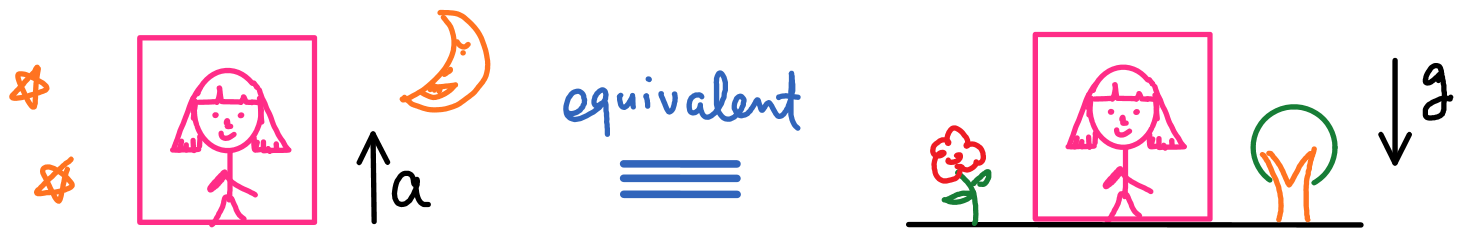
\includegraphics[width=1\textwidth]{ep}

    \tenum{
        \item 在没有重力的环境中电梯具有恒定加速度 $a$ 的升力
        \item 电梯没有移动,而是放置在引力场 $g=-a$ 中。
    }
    \tcblower
    我们在爱因斯坦的话中添加了“统一”以使其更加精确。如果引力场不均匀,我们总是可以研究空间中足够小的空间元素,其中引力场是均匀的。 (如何将这些小元素“拼凑”在一起很重要;这会导致时空弯曲。)
    \mtextbox{为什么作出这个假设}{每个人都可以做出假设。为什么这个是特别的?这个假设有着双重意义:
    \mtitem{
        \item 狭义相对论限制了我们对惯性系的关注。加速框架拓宽了相对论的范围。
        \item 重力从``常规''力降级为从根本上等同于虚构惯性力的东西。
    }}
}
这个假设确实回答了以下问题:$m_I=m_G$ 因为惯性(加速度)等于重力。引力是特殊的,因为这是这个基本假设中的力。


在这里,我们列举了一些假设的简单结果,并将更令人惊讶的结果留在后面的部分,因为它们需要更多的说明。

\textbox{匀加速可以抵消均匀重力}{
     这是因为均匀重力$g$等价于恒加速度$a=-g$,恒加速度$-g$可以被恒加速度$g$抵消。
    
    例如,人们在自由落体升降机或绕地球运行的卫星中感觉不到重力。这些观察者实际上可以将自己视为惯性系。对于这些观察者来说,均匀重力场可以被认为是不存在的(因为它不能被任何实验探测到)。

    因此(均匀)重力确实是特殊的(与所有其他力,如 E\&M 相比)——它和惯性力一样虚构。它的存在(或不存在)取决于观察者。
}
\mtextbox{星星、光线弯曲和透镜}{
    For a similar reason, light also bends when travelling near an object, such as a star, or a galaxy. One cannot compute the bending angle only from the equivalence principle since the gravitational field from a star is not uniform. From a calculation in general relativity, the bending angle is twice of naively applying the equivalence principle. This bending angle is the first verified prediction of general relativity (1915).出于类似的原因,光在靠近物体(例如恒星或星系)时也会弯曲。由于恒星的引力场是不均匀的,因此不能仅根据等效原理来计算弯曲角。根据广义相对论的计算,弯曲角度是天真地应用等效原理的计算结果的两倍。这个弯曲角度是广义相对论的第一个验证预测(1915)。
    \mnewline
    也可以另一种方式观察光线弯曲效果:物体像镜头一样聚焦光线。这种效应被称为 \textit{引力透镜}\index{引力透镜}。引力透镜被很好地观察到,并已成为了解我们宇宙物质分布的有力工具。
}
\textbox{光在均匀重力下弯曲\index{光的弯曲}}{
    光在均匀引力场中如何运动?这个问题在牛顿力学中可能被认为是没有明确定义的,因为光的质量为零(在相对论中,只有零质量的物体才能以有限的能量以光速运动)。但是根据等效原理,我们立即知道光的弯曲方式与加速环境中的弯曲方式相同。这解释了本部分开头的事例\ref{item:person-short} 。
}

\section{均匀重力时间}

回想一下,在孪生悖论中,加速会产生王二和王三之间的物理时间差(因为王二必须加速返回才能再次见到王三)。现在加速度等于均匀重力,我们预计重力也会在观察者之间造成一些时间差异。我们将看到情况确实如此。

\textbox{更高即更远}{
    现在王二比王三高一个垂直距离$h$。重力加速度为 $g$。王二的时间流逝和王三的时间流逝有什么不同吗?
    
    为了量化``时间流逝'',考虑王二发送两个间隔为 $\Delta t_A$ 的光脉冲。王三收到这两个脉冲的时间间隔是多少?

    为了更简便地计算,我们假设 $c\Delta t_A \ll h$ 和 $gh\ll c^2$。这种情况如下图的左侧面板所示。

    \cg{0.6}{ep_time}

    \tcblower
    
    为了解决这个问题,我们利用了等价原理。该系统相当于下图右侧面板中的情况:没有重力。而是王二和王三以加速度 $a=g$ 向上加速。
    
    我们设$t=0$为王二发出第一个信号的时间,也是王二和王三速度$v=0$的时间。让光信号的空间分离为$s$。请注意,$s$ 应该是一个常数,因为没有重力或其他影响光传播的力。

    关于王二,当她发送信号时,她的速度是 $v=0$,因此 $s= c\Delta t_A$。

    \marginnote{我们在王三的位置请了第三位观察者C静止研究王三关于光信号的运动。如果要说王三的时间间隔是什么,其实她和观察者C之间是有时间膨胀效应的。但是时间膨胀效应是$v^2/c^2$级的,所以在这个分析中很小。}
    关于观察者关于王三的位置是静置的,当王三接收到信号时,他的速度为 $v = a h/c$。请注意,光信号和王三正在朝着对方移动。因此$s = (c+v)\Delta t_B$。因此
    \begin{align}
        \Delta t_A = \left ( 1 + \frac{ah}{c^2}  \right ) \Delta t_B~.
    \end{align}
    因此,王三发现王二更快。王二越高越快。如果在$t=0$ 王二 和王三的年龄相同,之后王二会发现王三更年轻,王三会发现王二更老。

    这解释了本部分开头的事例 \ref{item:high-fast}。
}

\mtextbox{再次出现孪生悖论}{现在我们可以使用旅行双胞胎的框架来解释双胞胎悖论。旅行中的双胞胎需要在返回前加速。如果我们将加速度建模为匀加速,那么由于等效原理,对应于引力势。然后静态双胞胎在这种引力势中就突然变老了。}
\textbox{具有引力势的时间膨胀}{\index{引力时间膨胀}
    更一般地说,对于处于引力势 $\phi$ 中的王二和王三,时间膨胀可以用它们的引力势差表示为
    \begin{align}\label{eq:gr-phi}
        dt_A = \left ( 1 + \frac{\phi_A - \phi_B}{c^2}  \right ) dt_B ~.
    \end{align}
}


\textbox{球形恒星的度量}{\index{引力时间膨胀}
    Consider a spherical star with mass $M$. Let 王三 be at $r\rightarrow \infty$, i.e. far away from the star. Then 王三 does not experience gravity from the star, and has $\phi_B=0$. We can thus regard 王三's time as standard time without the star gravity: $t_B = t$.考虑质量为 $M$ 的球形恒星。令王三在 $r\rightarrow \infty$,即远离恒星。那么王三没有受到来自恒星的引力,并且有$\phi_B=0$。因此我们可以将王三的时间视为没有恒星引力的标准时间:$t_B = t$。
    
    While 王二 has gravitational potential $\phi_A=-GM/r$. Using Eq.~\eqref{eq:gr-phi}, we get\marginnote{Note that the gravitational field by the star is not uniform. But fortunately Eq.~\eqref{eq:gr-phi} can still be used here. And this even holds when gravity is very strong. The explanation (solving Einstein equations for the star) is beyond the scope of this short introduction.}而王二具有引力势$\phi_A=-GM/r$。使用方程~\eqref{eq:gr-phi},我们得到\marginnote{注意,恒星的引力场是不均匀的。不过好在 Eq.~\eqref{eq:gr-phi} 在这里还是可以用的。这甚至在重力非常强的情况下也成立。解释(解出恒星的爱因斯坦方程)超出了这个简短介绍的范围。}
    \begin{align}
        dt_A = \left ( 1 + \frac{\phi_A}{c^2}  \right ) dt~.
    \end{align}
    For 王二 static at a fixed position wrt the star, $d\mathbf{x}=0$, and对于王二静止在恒星的固定位置,$d\mathbf{x}=0$,并且
    \begin{align}
        \label{eq:ds2-schwarzschild}
        ds^2 = - c^2 (\mbox{proper time})^2  = - c^2 dt_A^2 
        = - \left ( 1 + \frac{2\phi_A}{c^2}  \right ) c^2 dt^2~. 
      \end{align}
      \mtextbox{Acceleration and spatial curvature}{
          Einstein noted that to reconcile accelerated frame and special relativity, the concept of curved 3d space has to be introduced. For example, consider 王二 experiencing uniform circular motion, and 王三 standing still at the center of the circle. 王二 and 王三 agrees on the radius of the circle, but not the circumference. Thus, 王二's space should be curved.爱因斯坦指出,为了协调加速坐标系和狭义相对论,必须引入弯曲 3d 空间的概念。例如,王二在做匀速圆周运动,王三站在圆心。王二和王三在圆的半径上一致,但在圆周上不一致。因此,王二的空间应该是弯曲的。
          \tcblower
          In curved space, say, a sphere, you can draw a draw a triangle and measure the sum of the inner angles. What do you get? That explains item \ref{item:inner-angle} at the beginning of this part.
      }
      In general, the coefficient in front of $d \mathbf{x}^2$ (i.e. the spatial part of the metric) is also modified. We will only give the result here: \index{Schwarzschild metric}
      \begin{align}
        \label{eq:schwarzschild}
        ds^2 = - \left ( 1 - \frac{r_s}{r}  \right ) c^2 dt^2
        + \left ( 1 - \frac{r_s}{r}  \right )^{-1} dr^2
        + r^2 \left ( d\theta^2 + \sin^2\theta d\phi^2 \right )~,
      \end{align}
      This is known as the Schwarzschild metric, describing the spacetime geometry outside a spherical symmetric star. The 这被称为 Schwarzschild 度量,描述了球对称恒星外部的时空几何。它的半径
      \begin{align}
        \label{eq:rs}
        r_s \equiv \frac{2GM}{c^2} 
      \end{align}
      is called the Schwarzschild radius.被称为史瓦西半径。
}

\textbox{Example: The sun}{
    To put in numbers for Eq.~\eqref{eq:rs}, if $M$ is the solar mass, then $r_s = 3$km. What does this 3km distance mean to the sun?为公式~\eqref{eq:rs} 代入数字,如果$M$ 是太阳质量,则$r_s = 3$km。这 3 公里的距离对太阳意味着什么?

    \tcblower

    It does not mean anything. Because the solar radius is $r_\odot = 7\times 10^5$km. The Schwarzschild metric \eqref{eq:schwarzschild} only applies outside the star, since inside the star, the form of gravitational potential takes a different form.

    However, what if an object is so dense, that its radius is smaller than $r_s$? For example, what if an object has the same mass of the sun, but with a radius smaller than 3km?
}

\section{黑洞}

Now imagine an object being so dense that its size is smaller than its Schwarzschild radius $r_s = 2GM/c^2$. What happens?

In fact, this is not a question living in imagination. Such dense objects -- black holes -- are real. They are detected from many observational methods, from the analysis of celestial motion to imaging its shape, to the observation of gravitational waves.

\textbox{What happens near $r=r_s$?}{
    When $r\simeq r_s$, in Eq.~\eqref{eq:schwarzschild} the time part vanishes and the spatial part blows up. What's happening there?

    Imagine 
    \mtextbox{Duality and holography}{Similar to the twin paradox, now 王二 and 王三 has a disagreement. 王二 sees herself falling across $r_s$ but 王三 sees 王二 frozen at $r_s$. We will explain that they do not have a chance to meet (up to quantum subtleties which remain open questions in research) and thus nothing goes wrong.
    \mnewline
    王三 sees and describes 王二 on the 2-dimensional surface $r=r_s$, while 王二 sees and describes herself in a 3-dimensional volume $r<r_s$. The two descriptions \textit{may} be equivalent to each other. This conjecture is known as holography in theoretical physics as the dual descriptions are between a surface and a volume.
    }
    that 王二 is staying at a distance $r$ very slightly greater than $r_s$. Gravity pulls her to fall but imagine that she is in a powerful rocket to keep her staying at a fixed $r$. And 王三 locates at $r\rightarrow \infty$. For any finite interval $\Delta t_A$ according to 王二, wrt 王三:
    \begin{align}
        \Delta t_B = \Delta t_A \times \left ( 1 - \frac{r_s}{r}  \right )^{- \frac{1}{2} } \rightarrow \infty~.
    \end{align}
    Thus, 王三 finds 王二 frozen on the $r=r_s$ surface. In general, at $r \rightarrow r_s$, the gravitational dilation effect is so significant that time looks frozen wrt an outside observer. In this respect, if you travel close to $r\rightarrow r_s$ and then back, it's a time machine that brings you to the future.
    \tcblower
    The above is what 王三 finds. But wrt 王二, she does not find $r=r_s$ very special. As at any moment, assuming that she is much smaller than $r_s$, equivalence principle tells that her acceleration cancels her gravity and she just crosses $r=r_s$ from outside to inside with finite time.
}

\textbox{An ``event horizon'' and a ``black hole''}{
    What will 王三 see for the events with $r<r_s$? For example, after 王二 crosses $r_s$ to reach $r<r_s$, what can 王三 see about 王二?

    Nothing. 
    \mtextbox{Are black holes really black?}{
        No.
        \tcblower
        \mtitem{
            \item Theoretically, Hawking radiations from quantum gravity can come out of black holes. They are usually too dim to see.
            \item Practically, some black holes are the brightest objects in our universe -- seriously. Matter falling into the black hole (infinitely deep gravitational potential) interact with each other and emit bright radiations -- up to $40\%$ of matter energy can be converted to light. Due to the emission of infalling matter, images of black holes have been taken by arrays of radio telescopes in 2019.
        }
    }
    Due to the extreme time dilation, the light emitted at $r_s$ need infinite time to reach 王三. 王三 does not have more than infinite time to wait and thus cannot see anything happening at $r<r_s$.

    As a result, $r=r_s$ is a surface to limit the events that 王三 can see. Thus, $r=r_s$ is known as an \textit{event horizon}\index{event horizon}. The dense object hides inside this event horizon and thus is invisible. No light from this object can reach to outside. Thus, the object is known as a \textit{black hole}\index{black hole}. This explains item \ref{item:black-horizon} at the beginning of this part.
}
 
\textbox{``Inside'' the horizon: the future is doomed at a singularity}{
    What happens after 王二 falls inside a black hole (cross the $r=r_s$ horizon)?王二掉进黑洞(穿过$r=r_s$视界)后会发生什么?

    Wrt 王三, he cannot expect to see 王二 coming out again. Since when she crosses the horizon, it already corresponds to $t_B\rightarrow \infty$. 王三 can see nothing happening later than infinity.

    But wrt 王二 herself, why cannot she decide to power her rocket to escape the horizon?
    \tcblower
    To answer this question, let us take a look at the Schwarzschild metric \eqref{eq:schwarzschild}. At $r<r_s$, the metric can be rewritten as
    \begin{align}
        \label{eq:schwarzschildIn}
        ds^2 = 
        - \left ( \frac{r_s}{r} -1 \right )^{-1} dr^2
        + \left (  \frac{r_s}{r} -1  \right ) c^2 dt^2
        + r^2 \left ( d\theta^2 + \sin^2\theta d\phi^2 \right )~.
    \end{align}
    \marginnote{This explains item \ref{item:singularity} at the beginning of this part.}
    What happened? Now $dr$ is time-like and $dt$ is space-like! The time direction and one space direction have flipped their roles. For 王二, the $-r$ direction is now the time direction.

    The time direction is special since it is one-way. You can choose to move left or right in space, but have no choice but moving forward in time. Now 王二 has no choice other than to move along her time direction (the direction to reduce $r$) towards $r=0$, regardless the spatial direction (now $t, \theta, \phi$) that 王二 would like to travel.

    Not only 王二, but everything inside the black hole, including the dense object itself, falls towards the future at $r=0$. Their time ends here and thus it is known as a \textit{singularity}\index{singularity}. In fact, following calculations of general relativity, before reaching the singularity, every object is teared apart due to diverging tidal force near the singularity. 

    Inside a black hole, the singularity is inevitable in classical general relativity. It remains an open question how this singularity can be resolved or understood in a complete theory which can describe gravity and quantum mechanics in a consistent way (quantum gravity).
}

\section{引力波}\index{gravitational waves}

Gravitational waves are consequences of the full theory of general relativity. Deriving them rigorously is beyond the scope here. We nevertheless build some intuitive understandings.引力波是广义相对论完整理论的产物。严格地推导它们超出了这里的范围。尽管如此,我们还是建立了一些直观的理解。

\textbox{Special relativity and Newtonian gravity are inconsistent}{
    What's wrong with the good old Newtonian gravity $F = G_N Mm / r^2$?

    Suppose 王二 is a light year away from 王三 and she waves her hand. As the position $r$ of her hands change, 王三 can in principle measure a slightly different gravitational attraction from 王二 \emph{immediately} -- because force needs no time to propagate in Newtonian gravity. 王二 can thus encode information in how her hands move, and the information is sent to 王三 immediately, which is faster than light.假设王二距离王三一光年,她挥手。随着她手的位置 $r$ 的变化,原则上王三可以测量出与王二 \emph {immediately} 略有不同的引力——因为力不需要时间在牛顿引力中传播。王二因此可以将信息编码在她的手如何移动中,并立即将信息发送给王三,这比光还快。

    From special relativity, no information can travel faster than light. Thus, Newtonian gravity is not consistent with special relativity.从狭义相对论来看,没有任何信息可以比光速传播得更快。因此,牛顿引力不符合狭义相对论。

    Conceptually, replacing gravity by spacetime curvature does not solve this problem -- can the spacetime curvature change with a speed faster than light when you move your hands?从概念上讲,用时空曲率代替重力并不能解决这个问题——当你移动你的手时,时空曲率是否能以比光还快的速度变化?
}

\mtextbox{引力波的早期历史}{
    Back to 1893, Oliver Heaviside noted the similarity of gravity and E\&M, and suggested that gravity may propagate in waves. But only after the estabilishment of general relativity, the discussion of gravitational waves was put into the approprate scientific framework. Einstein was the first to predict gravitational waves in 1916 based on his general relativity.回到 1893 年,Oliver Heaviside 注意到引力和 E\&M 的相似性,并提出引力可能以波的形式传播。但只有在广义相对论建立后,引力波的讨论才被纳入适当的科学框架。爱因斯坦于 1916 年第一个根据他的广义相对论预测了引力波。
}
\textbox{What gravity can learn from E\&M?从 E\&M 中可以学习到什么引力?}{
    In Newtonian gravity, you can send superluminal information by waving your hands and detect the force change using $F=G_N Mm /r^2$. However, why don't E\&M have the same problem with Coulomb force $F\propto Qq/r^2$?
    \tcblower
    If we only have the Coulomb force formula and nothing else, we would have the same superluminal problem for E\&M. However, the magnetic field comes to rescue here. Once the source electric charge accelerates (you cannot encode information by inertial motion without acceleration), the time variation of the electric field produces magnetic field, and the time variation of the magnetic field produces electric field. This process happens over and over again and E\&M wave is emitted at exactly the speed of light. Also, in this way, the E\&M field can propagate by itself without the need of matter (after produced by a source) as new ``degrees of freedom''.

    The lesson: we hope that new ``degrees of freedom'' can come to rescue in gravity, similar to what magnetic field does for E\&M. Where to find those degrees of freedom?
    % Internal note: The details: gravitoelectromagnetism. See for example:
    % https://arxiv.org/pdf/gr-qc/0003115.pdf
    % https://arxiv.org/pdf/gr-qc/9912027.pdf
}

\needspace{.22\textheight}
\mtextbox{Are gravitational waves physical?引力波是具有物质属性的吗?}{
     The concern is that space deforms, so does rulers. So can we actually measure gravitational waves? The debate lasted for 40 years. In 1957, Feynamn (under a pseudonym of ``Mr. Smith'') argued that when gravitational waves pass, a waterdrop on a rod will move wrt the rod and thus generate heat by friction. Thus gravitational waves are physical. The observational efforts start shortly afterwards. In 2016, after decades' trail and failure, gravitatioanl waves are finally detected by the Laser Interferometer Gravitational-Wave Observatory (LIGO) using an interferometer similar to the michelson morley experiment.令人担忧的是空间会变形,尺子也会变形。那么我们真的可以测量引力波吗?这场争论持续了 40 年。 1957 年,费南(化名“史密斯先生”)认为,当引力波通过时,棒上的水滴会相对于棒移动,从而通过摩擦产生热量。因此引力波具有物质属性的。观测工作随即开始。 2016 年,经过数十年的追踪和失败,引力波终于被激光干涉引力波天文台 (LIGO) 使用类似于迈克尔逊莫雷实验的干涉仪探测到。
}
\textbox{Optional: The dynamical metric and the gravitational waves可选(选读):动力学度量和引力波}{
    We have shown that a static gravitational field can be described by a non-trivial metric, for example \eqref{eq:schwarzschild}. There are other components in the metric as well. The metric can be viewed as a $4\times 4$ symmetric matrix with 10 components (free functions to choose). 8 of them are already used:
    \titem{
        \item 4 to describe the response to energy and momentum of matter. The energy part is the Newtonian gravity and the momentum part is its relativistic generalization. Technically they are called the Hamiltonian (energy) and momentum constraints.
        \item 4 represents the freedom to choose coordinates. When choosing any new coordinate system $\tilde x^\mu (x)$, we expect that the physical interval should not change and thus the metric should transform accordingly.
    }
    What are the remaining 2 degrees of freedom? Happily they correspond to propagating waves of gravity, to solve the problem of Newtonian gravity. And the gravitational waves propagate at the speed of light.
}

\marginnote{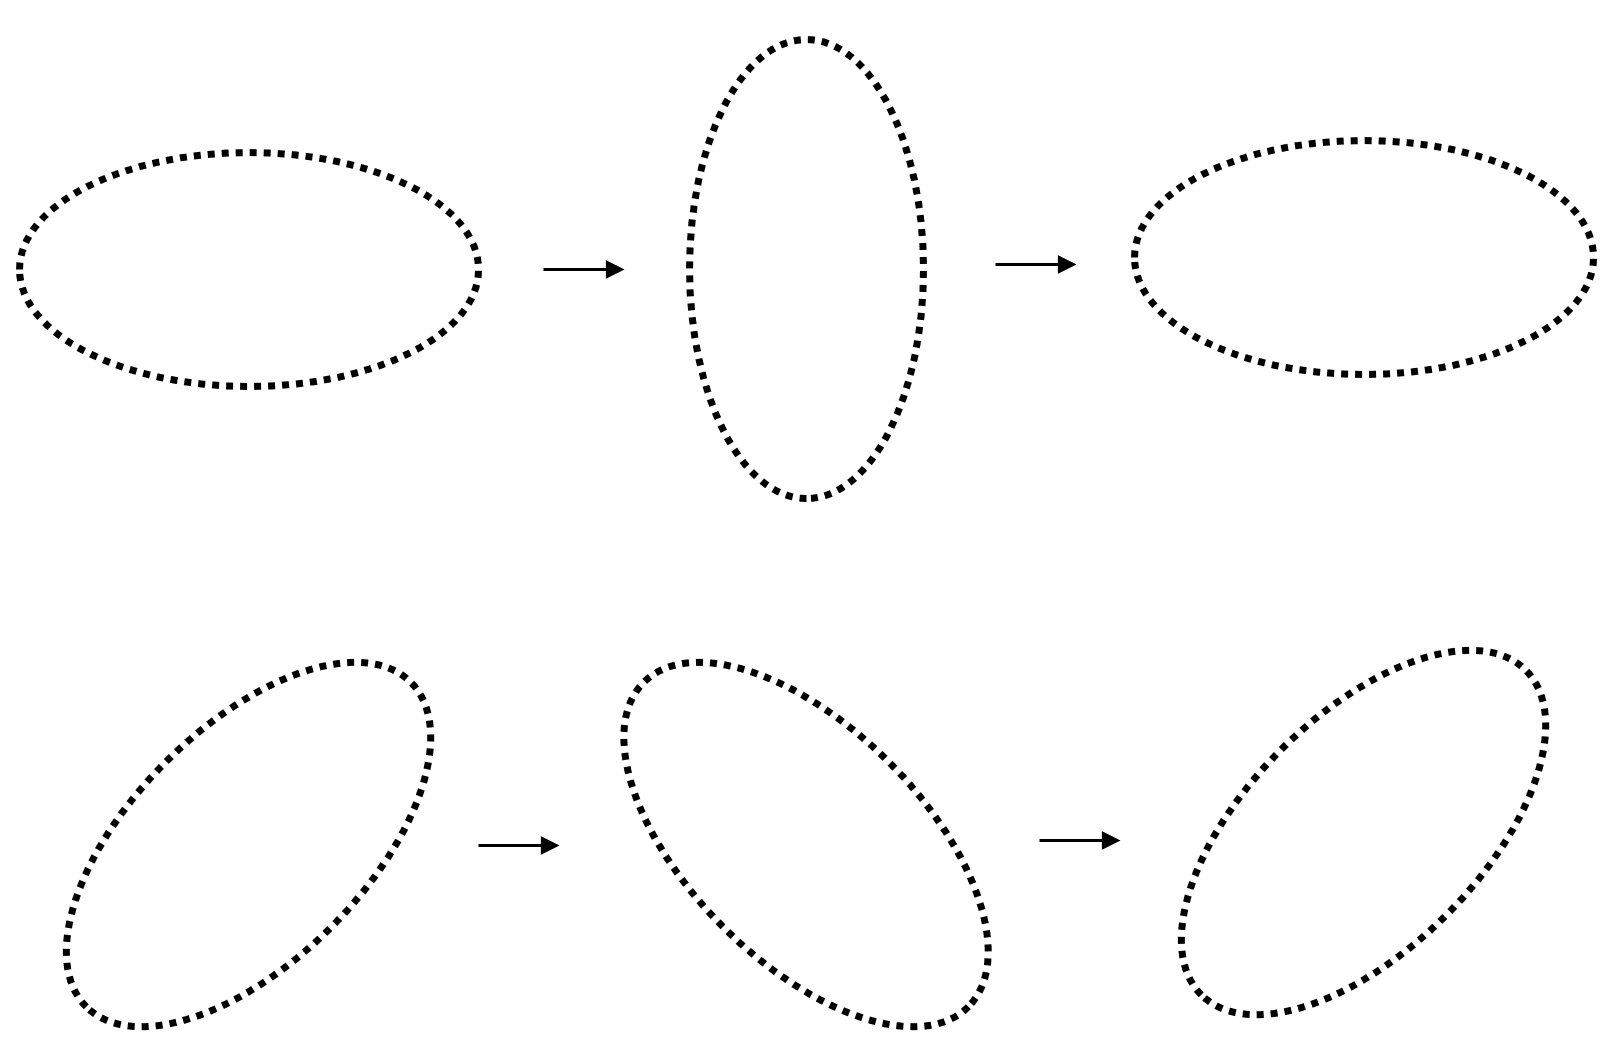
\includegraphics[width=0.35\textwidth]{gwpol}}
\textbox{What do gravitational waves look like?引力波是什么样子的?}{
    As we have argued, the gravitational waves are the fluctuations of spacetime, characterized by the metric. Thus, their impacts should be the distortion of distances. They travel at the speed of light and they are transverse waves (polarized perpendicular to the propagation direction). The two independent polarization modes deforms spacetime in the pattern sketched in the figure to the right.
}

\section{结语:总结和下一步}

\textbox{科学中罕见的例子}{
    广义相对论是现代科学史上一个非常罕见的例子,一个全新的科学框架。它(几乎)完全是由逻辑推理和哲学信仰建立的。

    Starts from the equivalence principle, we have shown you how time becomes relative in a uniform gravitational field. Then we argued that there is a similar effect for spherical stars. And if the star is dense enough, black holes form. The black hole has an event horizon where matter (classically, without the quantum mechanical considerations) can enter but not return. From the similarity between gravity and E\&M, we have argued that gravitational waves exist as deformations of spacetime. All these can be put into precise and elegant forms with the mathematical framework of differential geometry.从等效原理开始,我们向您展示了时间如何在均匀引力场中变得相对。然后我们认为球形恒星也有类似的效果。如果恒星足够密集,就会形成黑洞。黑洞有一个事件视界,物质(经典的,没有量子力学考虑)可以进入但不能返回。从引力和 E\&M 之间的相似性来看,我们认为引力波是作为时空变形而存在的。所有这些都可以用微分几何的数学框架精确而优雅地表达出来。
}

等效原理是广义相对论中的第一个观察结果,但这还不是最精彩的。虽然超出了课程的范围,但让我们提一下广义相对论中的两个关键概念:

\textbox{空间是如何弯曲的?}{
    How a geometry such as \eqref{eq:schwarzschild} is determined? In Newtonian gravity, we know that gravity is determined by matter distribution. Now that gravity is interpreted as geometry, geometry should be determined by matter distribution as well, at least in the Newtonian limit. The rule to determine geometry from matter distribution is the Einstein's equation. It looks like $G_{\mu\nu} = 8\pi G T_{\mu\nu}$ \index{Einstein's equations} and is the master equation of general relativity. I cannot explain it to you within the scope of this course, except mentioning that the LHS is determined by the metric $g_{\mu\nu}$ and its derivatives; and the RHS is determined by matter distribution. This is dubbed ``matter tells space how to curve.'' 如何确定诸如 \eqref{eq:schwarzschild} 之类的几何?在牛顿引力中,我们知道引力是由物质分布决定的。既然引力被解释为几何学,几何学也应该由物质分布决定,至少在牛顿极限内。从物质分布确定几何的规则是爱因斯坦方程。它看起来像 $G_{\mu\nu} = 8\pi G T_{\mu\nu}$ \index{爱因斯坦方程},是广义相对论的主要方程。我无法在本课程的范围内向您解释它,除非提到方程左侧由度量 $g_{\mu\nu}$ 及其衍生物决定;而方程右侧是由物质分布决定的。这被称为``物质告诉空间如何弯曲''。
}

\textbox{How matter moves?物质是如何运动的?}{
    How matter moves in curved space? Matter follows the geometry of spacetime. This is dubbed ``space tells matter how to move.'' Given a spacetime geometry, the motion of free-falling matter is determined by a generalized version of the twin paradox. Recall that in the twin paradox, the free observer without external force exerted has the longest proper time. We assert that, free-fall observers in general relativity still have extrema (usually longest but there are exceptions that the proper time is only longest for a selection of variations) proper times. Such extremal paths are known as geodesics. A geodesic can be interpreted in a semi-Newtonian manner as follows: the equation of a geodesic is物质如何在弯曲空间中运动?物质遵循时空的几何学。这被称为“空间告诉物质如何运动”。给定一个时空几何,自由落体物质的运动是由孪生悖论的广义版本决定的。回想一下,在孪生悖论中,没有施加外力的自由观察者的适当时间最长。我们断言,广义相对论中的自由落体观察者仍然具有极值(通常最长,但也有例外,正确时间仅对于选择的变体才是最长的)正确时间。这种极值路径称为测地线。测地线可以用半牛顿的方式解释如下:测地线的方程是 \index{geodesic equation} $a^\mu = - \sum_{\alpha,\beta=0}^3 \Gamma^\mu_{\alpha\beta} u^\alpha u^\beta$. Here $a_\mu$ is the 4-acceleration and $u^\alpha$ is the 4-velocity. $\Gamma^\mu_{\alpha\beta}$ is a generalization of the concept of gravitational force, made from the metric and its derivatives. You may have recognized that this looks like the Newton's second law. It is at your well whether to interpret the RHS as a gravitational force, or a term in geometry to tell matter how to move. They are equivalent as implied by the equivalence principle.$a^\mu = - \sum_{\alpha,\beta=0}^3 \Gamma^\mu_{\alpha\beta} u^\alpha u^\beta$。这里 $a_\mu$ 是 4-加速度,$u^\alpha$ 是 4-速度。 $\Gamma^\mu_{\alpha\beta}$ 是引力概念的推广,由度量及其导数构成。您可能已经认识到这看起来像牛顿第二定律。是否将RHS解释为重力,或几何学中的术语来说明物质如何运动,这完全取决于你。正如等价原则所暗示的那样,它们是等价的。
}

\textbox{Is general relativity general?广义相对论是广义的吗?}{
    The above two principles are the key to general relativity, which applies to all known scales where gravity can be studied, including millimeter scales for very precise gravity experiments in the lab, to the size of the whole universe.以上两个原理是广义相对论的关键,广义相对论适用于所有已知的可以研究重力的尺度,包括实验室非常精确的重力实验的毫米尺度,到整个宇宙的大小。

    Having that said, so far, we still do not understand how general relativity can be built within the framework of quantum mechanics. The efforts in searching for such a unified theory is known as ``quantum gravity''尽管如此,到目前为止,我们仍然不明白如何在量子力学的框架内建立广义相对论。寻找这样一个统一理论的努力被称为``量子引力''\index{quantum gravity}。Experiments have not been precise enough to probe quantum effects of gravity. But theoretical consistence between general relativity and quantum mechanics is also a well motived question, and is surprisingly hard. The current leading candidate of quantum gravity is string theory实验还不够精确,无法探测引力的量子效应。但是广义相对论和量子力学之间的理论一致性也是一个动机很好的问题,而且出奇地难。当前量子引力的主要候选者是弦论\index{string theory},它首先假设基本粒子实际上是一维空间而不是零维的弦(零对应于点粒子)。
} 

\textbox{扩展阅读}{
    有很多关于广义相对论的好书可以读。一些适合初学者的易读书籍有由Hartle\footnote{James B. Hartle(1939-),美国物理学家。——译者注。} 编写的 \href{https://www.amazon.com/dp/0805386629/?tag=stackoverfl08-20}{Gravity: An Introduction to Einstein’s General Relativity} 和 \href{https://www.amazon.com/First-Course-General-Relativity/dp/0521887054}{A First Course in General Relativity} by Schutz.
}


\section{练习}

1. 计算你在楼上变老的速度有多快。考虑狭义相对论和广义相对论的影响。

2. 考虑到现代卫星导航系统(如北斗、伽利略、GLONASS 或 GPS)的精度,如果不考虑这些因素,狭义相对论和广义相对论效应对这些卫星导航系统的精度有多大影响?

\printindex

\end{document} 